\chapter{Appendix: Explanation on Page Borders}\label{chap:appendix2}

What you find here is an explanation of why the border width keeps flipping from left to right -- which you might have spotted and wondered why that's the case.

Firstly, that is \emph{intended} and thus correct, so there is no reason to worry about this. The reason is that this document is configured as a two-sided book, which means:
\begin{compactitem}
  \item We assume the document will be printed out,
  \item that this will be done in a two-sided mode (i.e., the document will be printed on both sides of each page), and
  \item that the bookbinding will be in the middle, just like in every book.
\end{compactitem}

When you open the book, there are three borders of equal size~$n$. This however requires that even pages have a border of $n$ on their left and $\frac{n}{2}$ on their right, and odd pages have a border of $\frac{n}{2}$ on their left and $n$ on their right. This is illustrated in Figure~\ref{fig:pageBorders}.

\begin{figure}[h]
  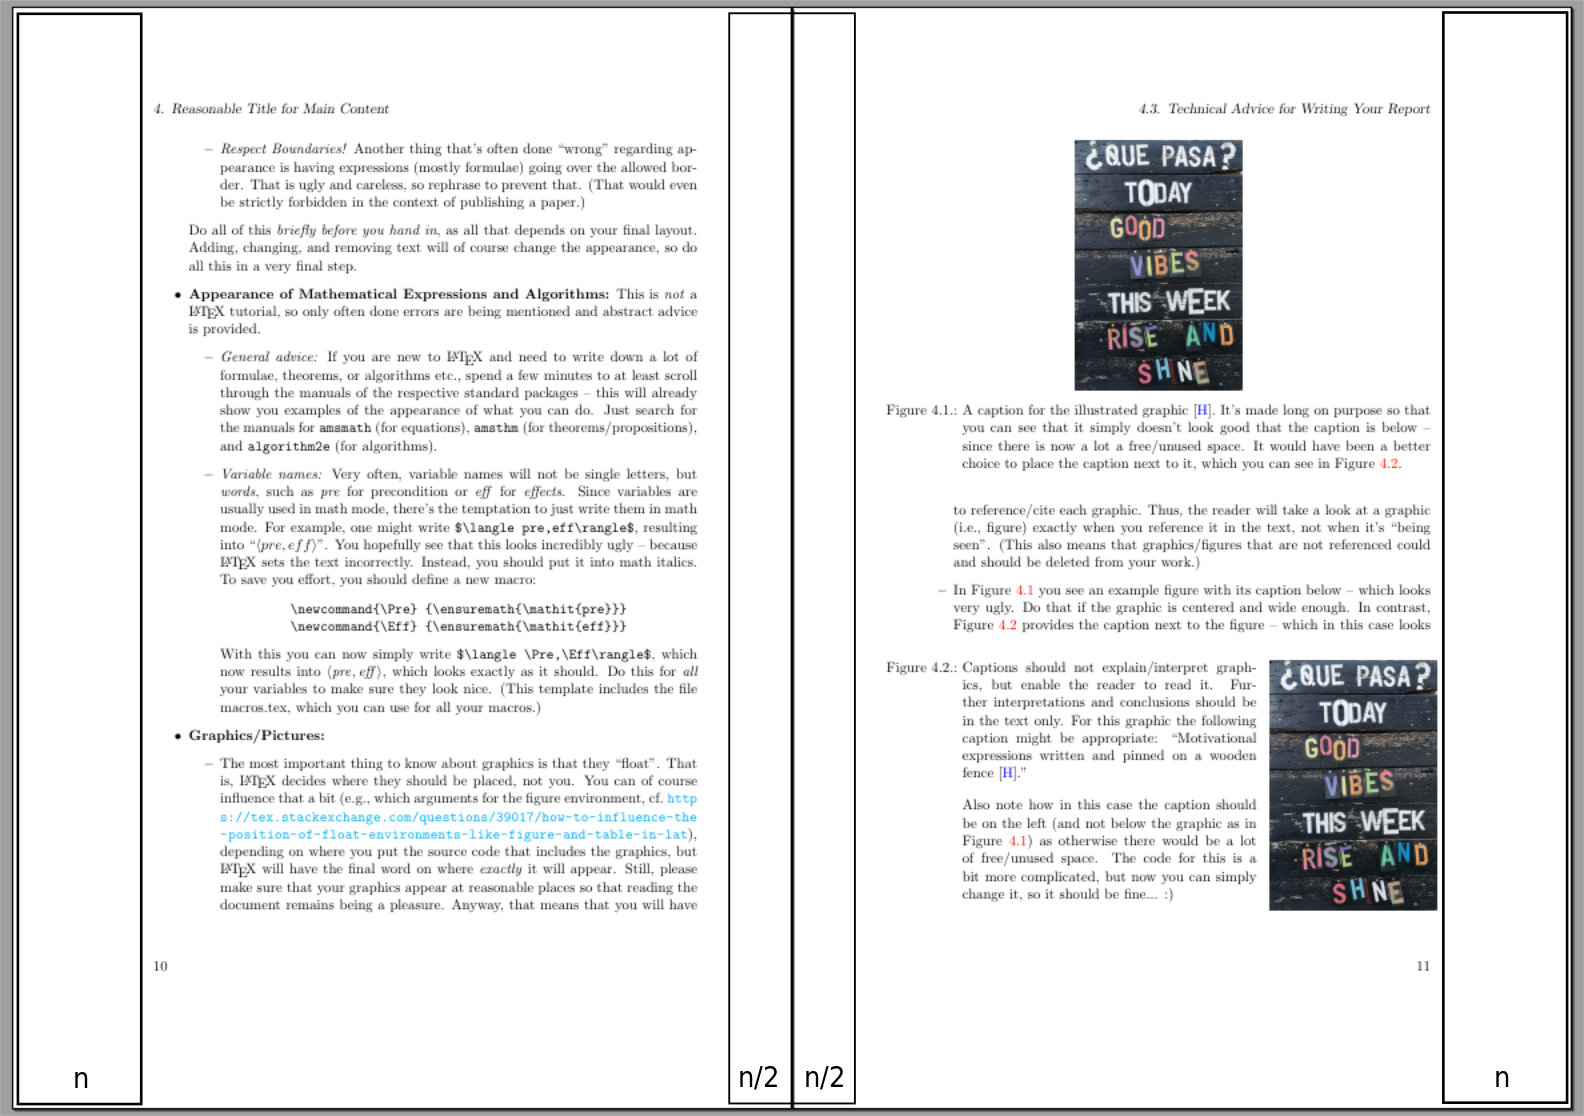
\includegraphics[width=.55\textwidth]{figures/borders--annotated}
  \caption{Illustration showing why page borders flip.\label{fig:pageBorders}}
\end{figure}%

